\section{La mise en œuvre du système}

\subsection{Tâches}

\begin{itemize}
	\item Création de l'architecture pour chaque composants(broker, subscriber, publisher)
	\item Choix des technologies qui seront utilisées et description des différences
	\item Exécution de l'esquisse du projet
	\item Implémentation en code des technologies choisies
\end{itemize}


\subsection{L'analyse du travail de laboratoire}

\textbf{\\Partie 1}\\

\emph{Création de l'architecture pour chaque composants(broker, subscriber, publisher) et l'écution de l'esquisse du projet}\\

\begin{figure}[!ht]
	\centering
	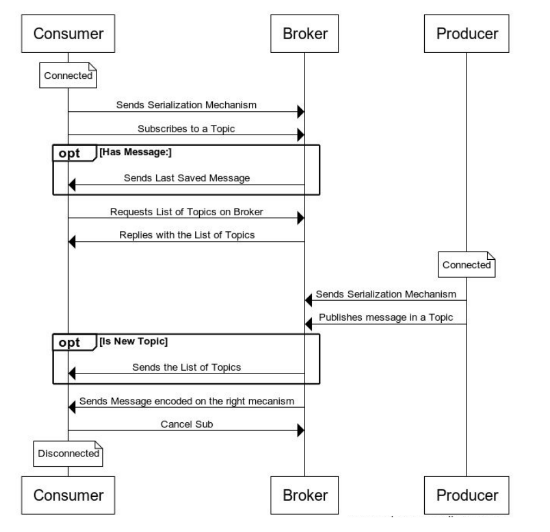
\includegraphics[scale=0.6]{structure}
	\caption{L'esquisse du projet}\label{structure}
\end{figure}
Donc, ici message Broker capable de relier les producteurs et les consommateurs via un protocole PubSub commun et des mécanismes de sérialisation ( JSON ) + middleware qui soustraient les producteurs et les consommateurs à l'ensemble du processus de communication.\\

\emph{Choix des technologies qui seront utilisées et description des différences}\\
\\• Protocole utilisé(TCP/UDP)\\
\\Le TCP permet aux systèmes de contrôler la livraison des paquets de deux façons. Premièrement, TCP numérote chaque paquet de manière à ce que le point de terminaison cible les rende dans le bon ordre. Deuxièmement, TCP comprend des mécanismes permettant de s’assurer que le point de terminaison cible reçoit chaque paquet de données.

Après avoir reçu un paquet, le dispositif destinataire(subscriber) renvoie un message à l’expéditeur(broker) pour accuser réception de la livraison. Si l’expéditeur ne reçoit pas de réponse du destinataire, l’expéditeur retransmet le paquet jusqu’à ce que le point de terminaison le reçoive avec succès ou annule les communications. Le TCP comprend également des fonctions de vérification d’erreurs pour s’assurer qu’aucune donnée n’est corrompue.

Malheureusement, toute cette fiabilité s’accompagne d’une surcharge importante, qui se traduit par une augmentation du nombre de transmissions, une demande accrue de la bande passante du réseau et un ralentissement général du traitement.
\\L’UDP résout ces problèmes en éliminant les contrôles et les équilibres du TCP, et en se concentrant uniquement sur la transmission des données. Il n’y a pas de numérotation des paquets, de vérification des erreurs ou d’accusé de réception de la livraison des paquets. Si les paquets se perdent lors de la transmission, ils restent perdus. Si les paquets sont hors service, ils le restent.
\\Alors, puisque nous avons un système de service, ou sont effectuées les transactions  et nous travaillons  avec les systèmes bancaires et les données personnelles des clients, le meilleur choix serait d'utiliser le protocole TCP afin de sécuriser et d'éviter la perte de données.\\
\\• Format de données (xml/json)\\\\
Pour les applications basées sur les données, je préfère utiliser JSON sur XML en raison de sa simplicité et de sa facilité de traitement côté client. XML peut être indispensable sur le serveur, mais JSON est définitivement plus facile à utiliser sur le client.\\
\\• Sockets/Asyncio\\
Il y en a moins qui se concentrent sur l'utilisation de sockets, pour écouter ou envoyer aux connexions. Comme nous visons à créer un serveur Web, le TCP (protocole) a du sens.
Asyncio propose deux choix de haut niveau pour l'écriture de serveurs, basés sur le rappel ou sur le flux. Je pense que ce dernier est conceptuellement plus clair, mais il a été démontré qu'il avait de moins bonnes performances.
Donc, nous avons décidé d'utiliser des sockets pour fournir un échange d'informations entre les processus qui se produira lors de l'utilisation des services de notre système.\\
\\• DB or not\\
Les bases de données NoSQL sont généralement dé-normalisées (en enregistrant une copie des données de l'objet au lieu de l'objet), tout comme une base de données normalisée OODB avec des relations d'objet. Dans un OODB, les données sont stockées dans un objet au même endroit et sont liées (liées) à d'autres objets.

En raison de la différence ci-dessus entre dénormalisé et normalisé, les deux ont leurs avantages et leurs inconvénients. Les bases de données NoSQL, comme Mongo, sont rapides en lecture mais pauvres en écriture / mise à jour des données. En raison de la nature dé-normalisée des bases de données NoSQL, il est difficile de maintenir l'intégrité des données là où OODB et Wakanda sont facilement gérés et ont l'intégrité des données. Lorsqu'un objet est supprimé et que tous ses liens sont supprimés automatiquement.
Nous allons donc essayer d'utiliser la base de données pour stocker des informations.\\

\textbf{Pattern Pub / Sub}

Comme base pour mener à bien cette mission, nous avons utilisé le pattern Publish-Subscribe, dans lequel les éditeurs (producteurs) publient des messages sur certains sujets, les éditeurs sont faiblement couplés aux abonnés (consommateurs) et n'ont même pas besoin de connaître leur existence, et chaque l'abonné qui s'est abonné à ces sujets recevra ces messages. Il a été mis en place une entité intermédiaire, un Broker, avec la fonction de transmettre les messages aux abonnés et de hiérarchiser les messages dans une file d'attente avant de les envoyer, chaque fois qu'un message était publié ou lorsqu'ils se connectaient avec le Broker (envoi du dernier Message) encodé Mécanisme de sérialisation puisqu'ils peuvent chacun avoir des mécanismes différents. Il présente également un middleware qui soustrait tous les producteurs / consommateurs du processus de communication.\\

\textbf{Flow/Architecture logicielle}

Lors de l'exécution de cette affectation, le flux de messages entre les entités présentes a obtenu la forme suivante, comme on peut le voir sur le Message Sequence Chart. Ces flux de messages seront expliqués au cours de ce rapport.\\


\textbf{Broker}

Dans son cœur, un courtier de messages est «un programme qui traduit un message en un protocole de messagerie formel de l'expéditeur, en protocole de messagerie formel du destinataire»\\
\textbf{\\Quand un courtier de messages est-il nécessaire?}\\
\begin{itemize}
	\item Si nous souhaitons contrôler les flux de données. Par exemple, le nombre d'inscriptions dans n'importe quel système.
	\item Lorsque la tâche est d'envoyer des données à plusieurs applications et d'éviter l'utilisation directe de leur API.
	\item Lorsque nous avons besoin de terminer des processus dans un ordre défini, comme un système transactionnel.
\end{itemize}
Ainsi, nous pouvons dire que les courtiers en messages peuvent faire quatre choses importantes:

\begin{enumerate}
	\item divisez l'éditeur et le consommateur (publisher and consumer).
	\item stocker les messages.
	\item messages d'acheminement (route messages).
	\item vérifier et organiser les messages.
\end{enumerate}
Eh bien, un broker de messages est vraiment bon dans une chose - traiter les messages.
Cela signifie que lorsque nous avons beaucoup de messages (pensez à des milliers, des millions, des milliards de messages), il pourrait être intéressant de consulter un broker de messages pour créer un magasin / processeur centralisé pour ces messages, afin que d'autres applications ou utilisateurs puissent travailler avec ces messages - notre seule source de vérité.\\

\textbf{Middleware}

Afin de savoir quel mécanisme de sérialisation est pris en charge par chaque entité côté middleware (producteur et consommateur), une fois que chaque file d'attente établit une connexion TCP avec le courtier, elle envoie un message avec son mécanisme sous forme de chaîne au courtier avant tout autre message est envoyé. Après cela, le Middleware sait encoder / décoder les messages car ces fonctions d'encodage et de décodage des données des différents mécanismes ont le même nom sur la classe représentative du mécanisme. Il en va de même pour Broker, car il aura enregistré le mécanisme du socket et saura quelles opérations utiliser.

Pour distinguer chaque type de messages envoyés par un consommateur / producteur, chaque message est encodé avec une méthode (Exemple: PUBLISH, SUBSCRIBE), topic (Exemple: Si nous voulons souscrire un certain topic, annuler un abonnement spécifique ou publier un message dans un sujet) et le dernier, mais non le moindre, le message lui-même. Cela permet de créer un type générique de «protocole» pour le codage et le décodage des messages. Nous avons décidé de faire l'abonnement du sujet passé comme argument de ligne de commande à chaque fois que nous exécutons un nouveau consommateur, car nous ne pourrions pas obtenir le même socket si la connexion avec le Broker se terminait.\\

\textbf{List Topics and Cancel Subscription Operation}

Notre approche pour lister les Topics consistait à envoyer tous les sujets courants (hors racine) présents sur Broker après la première opération d'abonnement et à chaque fois qu'un nouveau sujet était créé. Ce faisant, permet au consommateur de connaître les autres sujets qui existent dans le «canal» au moment du premier abonnement et également si un sous-sujet d'un sujet auquel l'utilisateur s'est abonné avait déjà été créé; les utilisateurs recevraient cette information avant tout message d'un éventuel nouveau sous-thème. Pour ce faire, nous avons créé une méthode dans le Middleware qui envoie un message au courtier demandant la liste initiale des sujets, le courtier répond avec une chaîne avec tous les sujets (en évitant les interruptions s'il a envoyé les sujets individuellement), après cela, c'est la responsabilité du courtier d'envoyer la liste des sujets à chaque fois qu'un nouveau sujet est créé.

Comme nous avons utilisé des sockets Python pour autoriser les connexions TCP requises, quand un socket se ferme, il est impossible de lui envoyer des informations par la suite, et par conséquent, notre implémentation a nécessité de supprimer des structures de données de notre courtier, ces sockets (en évitant d'envoyer à un connexion fermée). Tous ces points constituaient la base de notre opération d'annulation. Nous avons décidé d'annuler un abonnement dans deux scénarios possibles:

- Si nous voulons annuler un certain abonnement, nous supprimons uniquement le socket de ce sujet et, bien sûr, ses sous-sujets, en utilisant à nouveau regex;

- Si nous fermons une connexion, nous supprimons simplement le socket fermé de toutes les structures de données.

Pour tester ces scénarios possibles, nous avons imprimé côté Broker les données du dictionnaire topicmsg. Dans le dernier scénario, en utilisant une KeyBoardInterruptException dans le consommateur, la fonction cancelSub du côté Middleware a été déclenchée en passant le sujet consommateur en argument. Il est important de mentionner que même si le deuxième scénario se produit, nous supprimons toujours toutes les entrées de socket des structures de données Broker.\\

\textbf{Stratégie de validation de solution}

Après avoir implémenté notre approche à ce problème, nous sommes revenus à quelques tests, pour vérifier si tout fonctionnait comme il se doit. Pour tester les mécanismes de sérialisation des variables, nous avons utilisé, par exemple, la sérialisation des producteurs avec JSON Mechanism. L'évolutivité de notre solution, a été testée en exécutant un consommateur qui s'abonne à la racine («/») et 2 autres producteurs qui ont publié pour le sujet «/ telephony» et «/ msg», et par conséquent, nous parvenons à recevoir le messages. Les files d'attente FIFO semblent fonctionner correctement car si un nouveau consommateur s'abonne à un sujet où des messages avaient été envoyés, cette entité recevra le dernier message.


\textbf{\\Principe de fonctionnement de RabbitMQ :}\\
Créé en tant que broker de messages à usage général, RabbitMQ est basé sur le modèle de communication pub-sub. Le processus de messagerie peut être synchrone ou asynchrone, selon notre préférence.
Étant un programme centré sur les broker, RabbitMQ donne des garanties entre les producteurs et les consommateurs. Si vous choisissez ce logiciel, vous devez utiliser des messages transitoires plutôt que durables.

Le programme utilise le broker pour vérifier l'état d'un message et vérifier si la livraison s'est terminée avec succès. Le broker de messages suppose que les consommateurs sont généralement en ligne.

Quant à l'ordre des messages, les consommateurs recevront le message dans l'ordre publié lui-même. L'ordre de publication est géré de manière cohérente.
Nous aimons RabbitMQ en raison de la possibilité d'utiliser de nombreux plugins. Ils font gagner du temps et accélèrent le travail.
\begin{figure}[!ht]
	\centering
	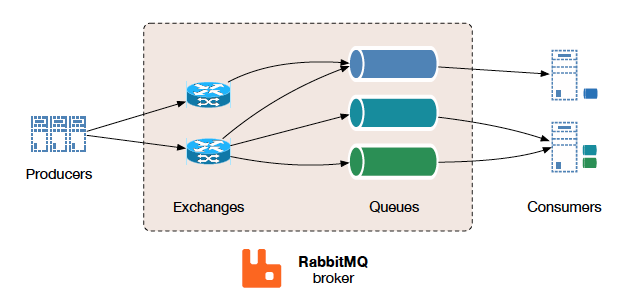
\includegraphics[scale=0.8]{rabbit}
	\caption{Architecture de RabbitMQ}\label{rabbit}
\end{figure}

\textbf{\\Partie 2}\\\\
Le système d'appel de procédure à distance (RPC) nous permet d'appeler une fonction disponible sur un serveur distant en utilisant la même syntaxe que celle utilisée lors de l'appel d'une fonction dans une bibliothèque locale. Ceci est utile dans deux situations.\\
Nous pouvons utiliser la puissance de traitement de plusieurs machines à l'aide de rpc sans changer le code pour appeler les programmes situés dans les systèmes distants.
Les données nécessaires au traitement ne sont disponibles que dans le système distant.
Ainsi, en python, nous pouvons traiter une machine comme un serveur et une autre machine comme un client qui appellera le serveur pour exécuter la procédure distante.

\textbf{\\Exécuter un serveur}\\\\
Le langage python est livré avec un serveur intégré que nous pouvons exécuter en tant que serveur local. Le script pour exécuter ce serveur est situé sous le dossier bin de l'installation de python et nommé classic.py. Nous pouvons l'exécuter dans l'invite python et vérifier son exécution en tant que serveur local.
python bin/classic.py
Lorsque nous exécutons le programme ci-dessus, nous obtenons la sortie suivante –
INFO:SLAVE/18812:server started on [127.0.0.1]:18812

\textbf{\\Exécuter un client}\\\\
Ensuite, nous exécutons le client à l'aide du module rpyc pour exécuter un appel de procédure à distance. Dans l'exemple ci-dessous, nous exécutons la fonction d'impression sur le serveur distant.
import rpyc
conn = rpyc.classic.connect("localhost")
conn.execute("print('Hello from Students')")
Lorsque nous exécutons le programme ci-dessus, nous obtenons la sortie suivante –
Hello from Students\\
\textbf{\\Évaluation des expressions via RPC}\\\\
En utilisant les exemples de code ci-dessus, nous pouvons utiliser les fonctions intégrées de python pour l'exécution et l'évaluation d'expressions via rpc.

\begin{verbatim}
	import rpyc
	conn = rpyc.classic.connect("localhost")
	conn.execute('import math')
	conn.eval('2*math.pi')
\end{verbatim}
Lorsque nous exécutons le programme ci-dessus, nous obtenons la sortie suivante –
6.283185307179586\\

La fonction readPubSub est l'une des fonctions les plus importantes du côté Broker. Comme cela rendrait le code répétitif pour certaines parties similaires dans les opérations de lecture / écriture, nous décidons de n'utiliser qu'une seule fonction capable de savoir s'il s'agit d'un message de publication ou d'abonnement. Si c'est un message de publication, il sera passé comme argument d'un msg, sinon le msg sera «Aucun». Pour itérer, nous avons utilisé regex afin de pouvoir diviser le sujet passé en argument et les concaténer un par un à chaque itération, ce qui constitue un moyen très rapide de faire l'opération de publication car la longueur de la «boucle for» sera toujours en fonction du nombre d'éléments que la méthode de fractionnement nous a donné et nous pouvons simplement insérer des messages tout de suite au bon endroit. Lors de l'itération, nous transmettons une liste d'utilisateurs du sujet à ses sous-sujets (en évitant toujours les informations en double).

Il est important de mentionner que nous avons utilisé une file d'attente FIFO pour les messages de chaque sujet, afin que nous puissions non seulement enregistrer le dernier message publié mais aussi pour éviter que deux producteurs envoient un message en «même» heure (le premier message arrivé sera envoyé en premier , puis est sorti de la liste). La pire partie de l'utilisation de regex pour implémenter cela, c'est dans l'opération d'abonnement en raison du fait que cela oblige à itérer le dictionnaire topicmsg pour voir si le sujet auquel le consommateur veut s'abonner contient des sous-sujets utilisant regex, ce qui peut être une opération très lente si le dictionnaire a une dimension considérable. Dans ce cas, une meilleure approche consisterait à utiliser une implémentation d'arbre non binaire pour les sujets en évitant une complexité de temps O (n) dans l'opération de recherche.\\

\textbf{\\L'étapes dans l'exécution du RPC :}\\\\
\begin{figure}[!ht]
	\centering
	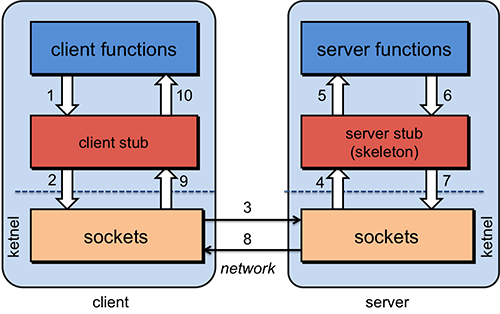
\includegraphics[scale=1.3]{step}
	\caption{Steps in executing a remote procedure call}\label{step}
\end{figure}

\begin{enumerate}
	\item[1.] Le client appelle une procédure locale, appelée le stub client. Pour le processus client, cela semble être la procédure réelle, car il s'agit d'une procédure locale régulière. Il fait juste quelque chose de différent puisque la vraie procédure est sur le serveur. Le stub client regroupe les paramètres dans la procédure distante (cela peut impliquer de les convertir dans un format standard) et génère un ou plusieurs messages réseau. L'empaquetage des arguments dans un message réseau s'appelle le marshaling et nécessite la sérialisation de tous les éléments de données dans un format de tableau d'octets plat.
	\item[2.] Les messages réseau sont envoyés par le stub client au système distant (via un appel système au noyau local à l'aide des interfaces de sockets).
	\item[3.] Les messages réseau sont transférés par le noyau vers le système distant via un protocole (sans connexion ou orienté connexion).
	\item[4.] Un stub de serveur, parfois appelé squelette, reçoit les messages sur le serveur. Il démarshale les arguments des messages et, si nécessaire, les convertit d'un format réseau standard en une forme spécifique à la machine.
	\item[5.] Le stub de serveur appelle la fonction serveur (qui, pour le client, est la procédure distante), en lui passant les arguments qu'il a reçus du client.
	\item[6.] Lorsque la fonction serveur est terminée, elle retourne au stub du serveur avec ses valeurs de retour.
	\item[7.] Le stub de serveur convertit les valeurs de retour, si nécessaire, et les rassemble en un ou plusieurs messages réseau à envoyer au stub client.
	\item[8.] Les messages sont renvoyés sur le réseau vers le stub client.
	\item[9.] Le stub client lit les messages du noyau local.
	\item[10.] Le stub client renvoie ensuite les résultats à la fonction client, en les convertissant de la représentation réseau en représentation locale si nécessaire.
\end{enumerate}
\textbf{\\Le code client continue alors son exécution.}\\\\
\emph{Les principaux avantages du RPC sont doubles. Premièrement, le programmeur peut maintenant utiliser la sémantique des appels de procédure pour appeler des fonctions distantes et obtenir des réponses. Deuxièmement, l'écriture d'applications distribuées est simplifiée car RPC masque tout le code réseau dans des fonctions de stub. Les programmes d'application n'ont pas à se soucier des détails tels que les sockets, les numéros de port, la conversion et l'analyse des données. Sur le modèle de référence OSI, RPC couvre à la fois les couches session et présentation (couches cinq et six).}

\textbf{\\Et la sécurité?}\\\\
C'est certainement quelque chose dont nous devons nous inquiéter. Avec les procédures locales, tous les appels de fonction sont dans les limites d'un processus et nous attendons du système d'exploitation qu'il applique une protection de mémoire adéquate via des mappages de mémoire par processus afin que les autres processus ne soient pas au courant de manipuler ou d'examiner les appels de fonction. Avec RPC, nous devons nous préoccuper de divers problèmes de sécurité:
\begin{itemize}[label=$\ast$]
	\item Le client envoie-t-il des messages au bon processus distant ou le processus est-il un imposteur?
	\item Le client envoie-t-il des messages à la bonne machine distante ou la machine distante est-elle un imposteur?
	\item Le serveur n'accepte-t-il que les messages de clients légitimes? Le serveur peut-il identifier l'utilisateur côté client?
	\item Le message peut-il être reniflé par d'autres processus pendant qu'il traverse le réseau?
	\item Le message peut-il être intercepté et modifié par d'autres processus pendant qu'il traverse le réseau de client à serveur ou de serveur à client?
	\item Le protocole est-il sujet à des attaques par rejeu? Autrement dit, un hôte malveillant peut-il capturer un message et le retransmettre ultérieurement?
	\item Le message a-t-il été accidentellement corrompu ou tronqué sur le réseau?
\end{itemize}
\hfill \break


\subsection{Les images}

\emph{\\Implémentation en code des technologies choisies et présentation de fonctionnalité du code}\\

\textbf{broker.py}
\begin{figure}[!ht]
	\centering
	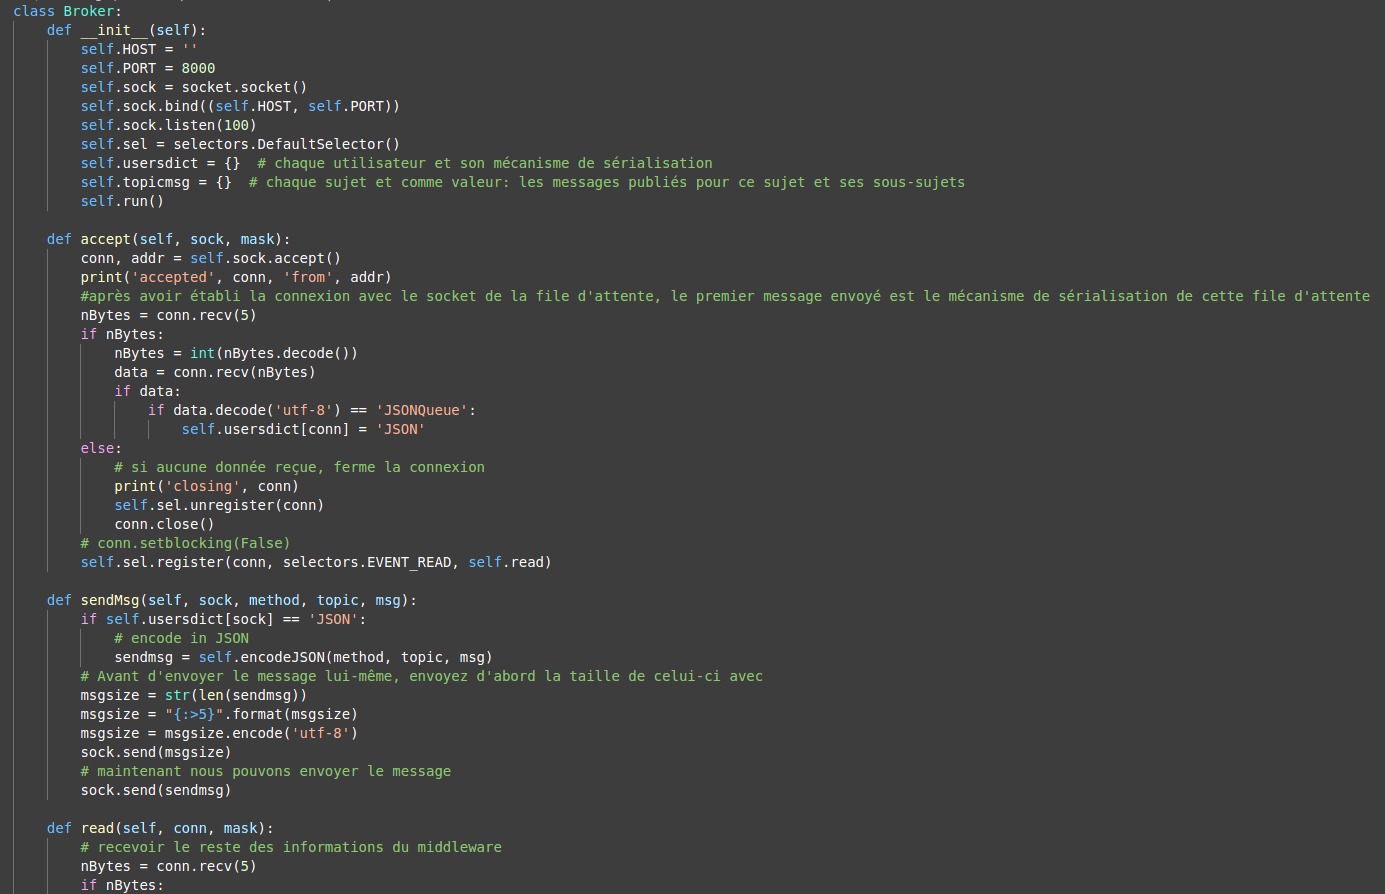
\includegraphics[scale=0.3]{b1}
	\caption{Broker part 1}\label{b1}
	\vspace{1cm}
	\centering
	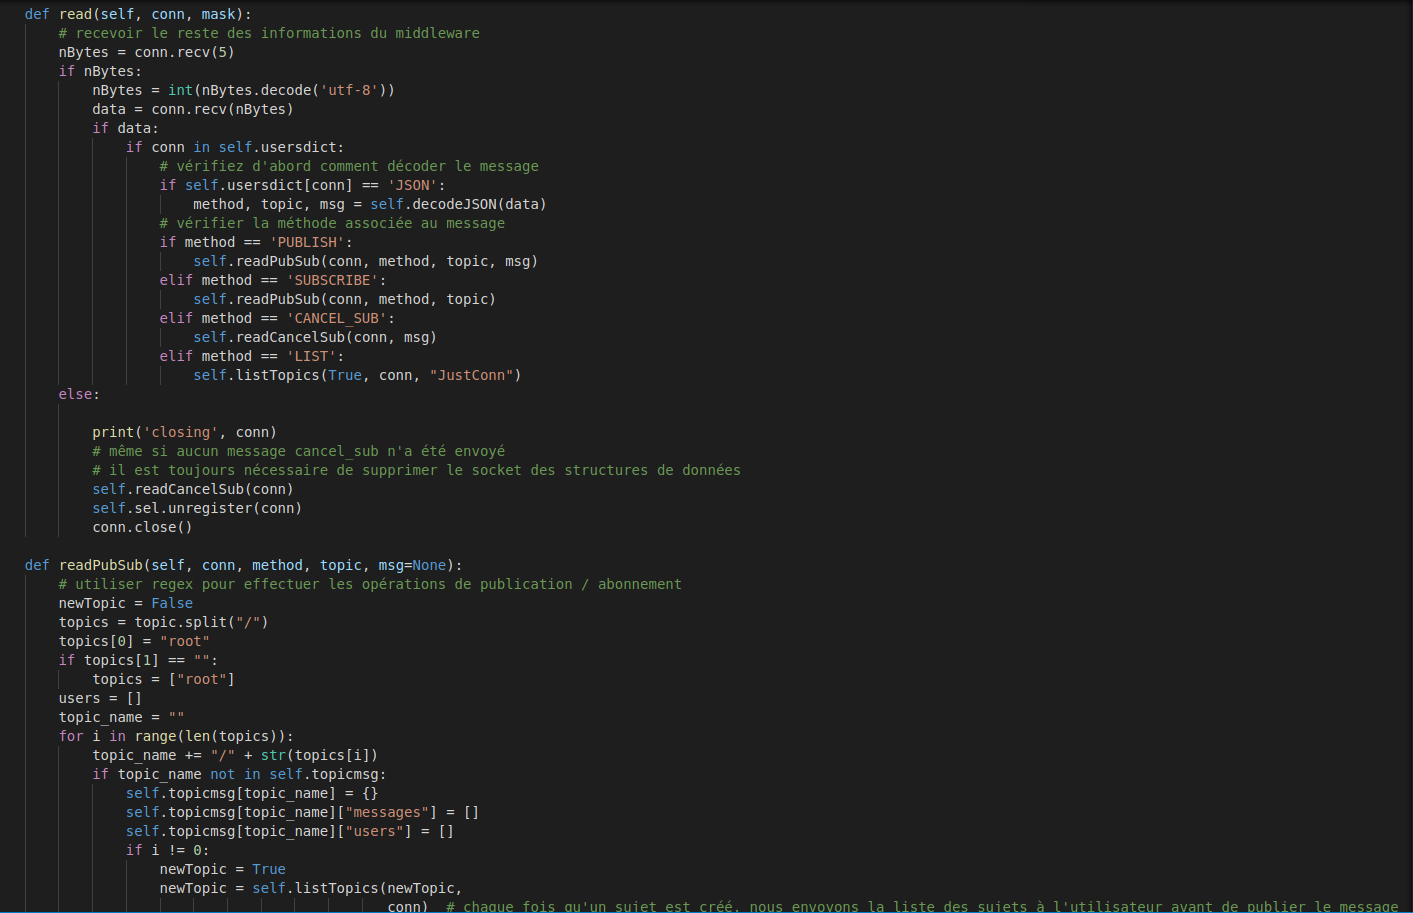
\includegraphics[scale=0.3]{b2}
	\caption{Broker part 2}\label{b2}
\end{figure}

\begin{figure}[!ht]
	\centering
	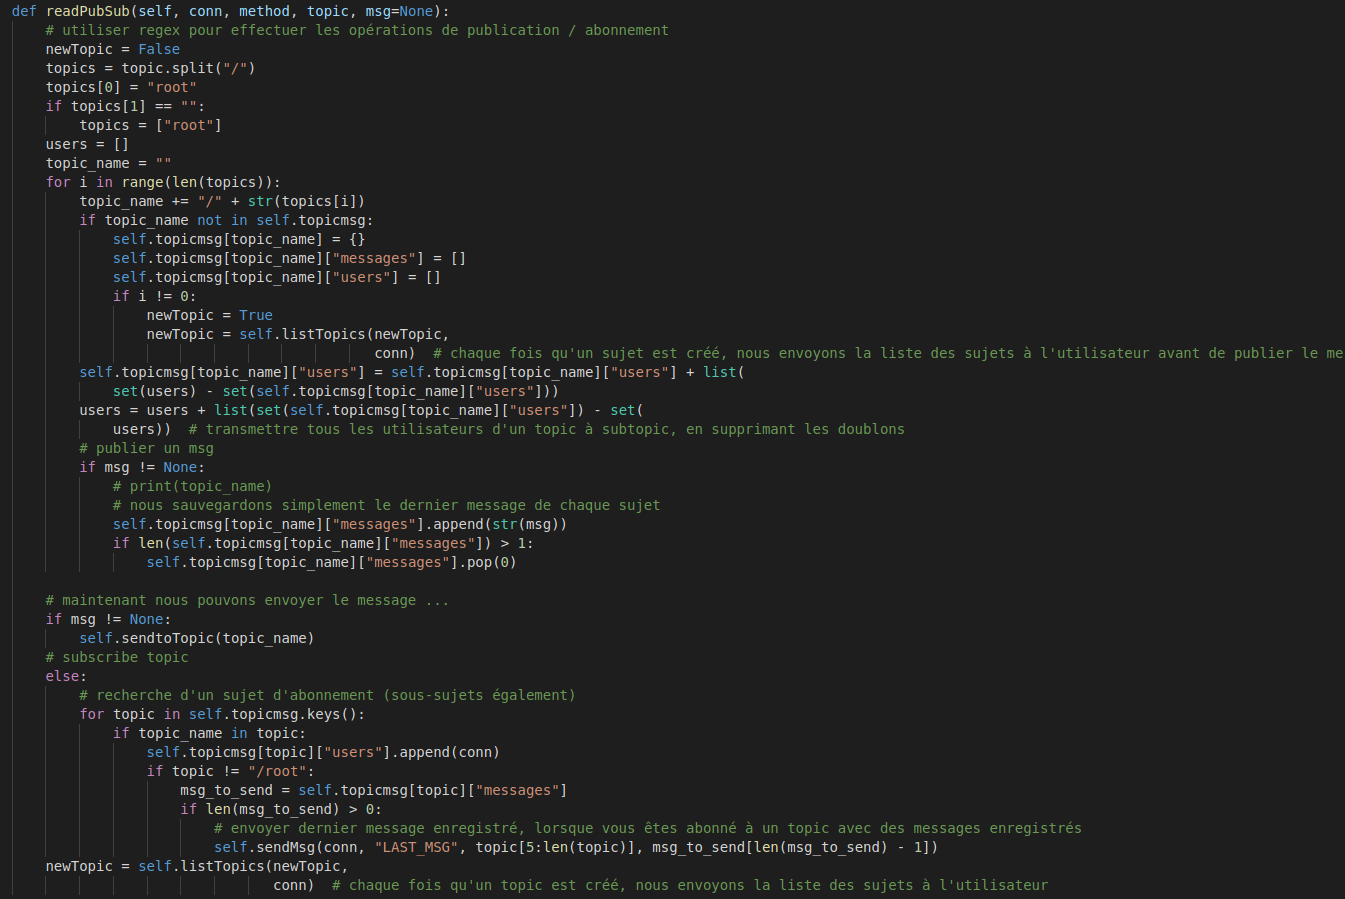
\includegraphics[scale=0.3]{b3}
	\caption{Broker part 3}\label{b3}
	\vspace{1cm}
	\centering
	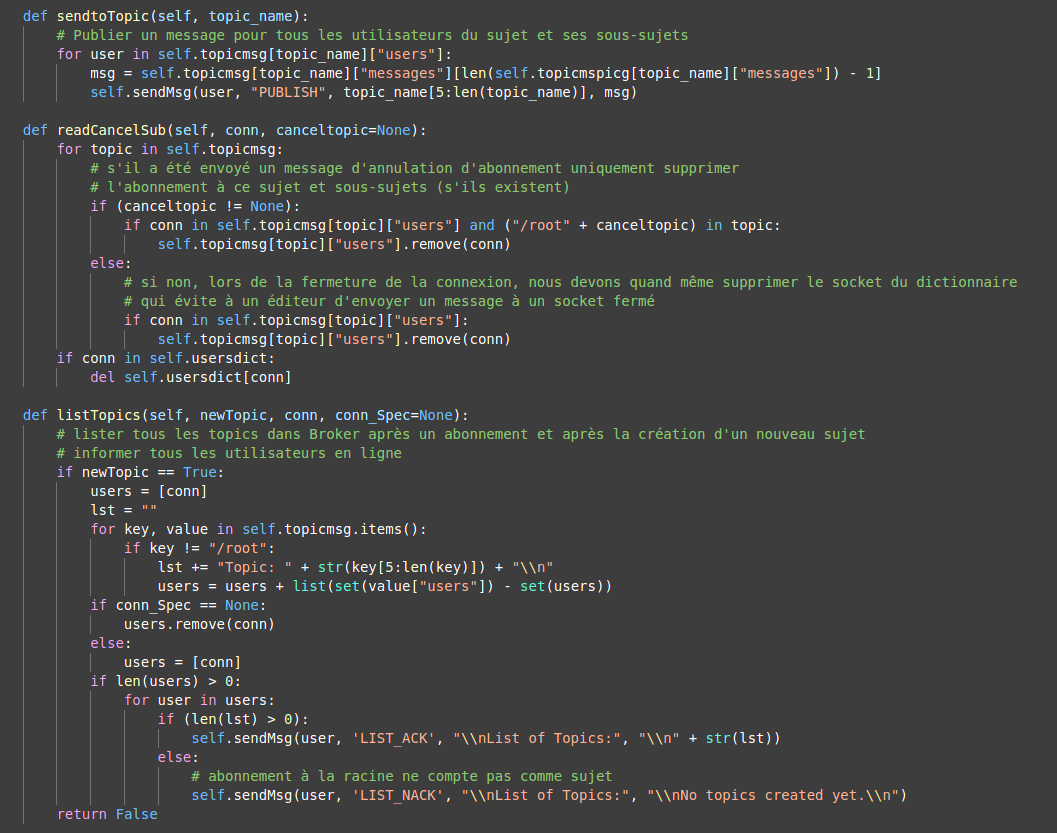
\includegraphics[scale=0.4]{b4}
	\caption{Broker part 4}\label{b4}
\end{figure}

Broker class \\\\\\\\\\\\\\\\\\

\textbf{\\middleware.py}\\
\begin{figure}[!ht]
	\centering
	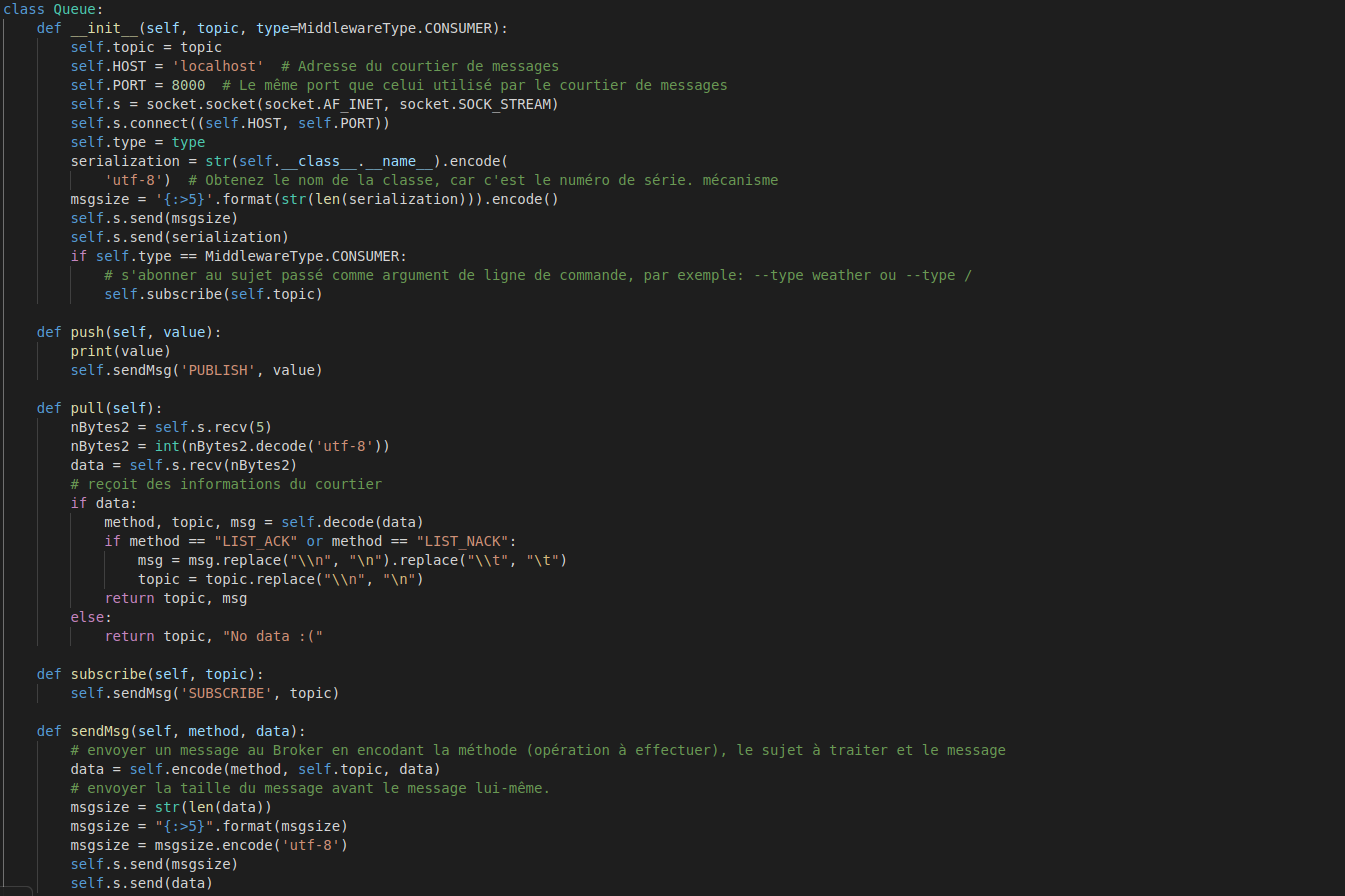
\includegraphics[scale=0.3]{middleware}
	\caption{middleware.py}\label{middleware}
\end{figure}


\textbf{\\producer.py}\\
\begin{figure}[!ht]
	\centering
	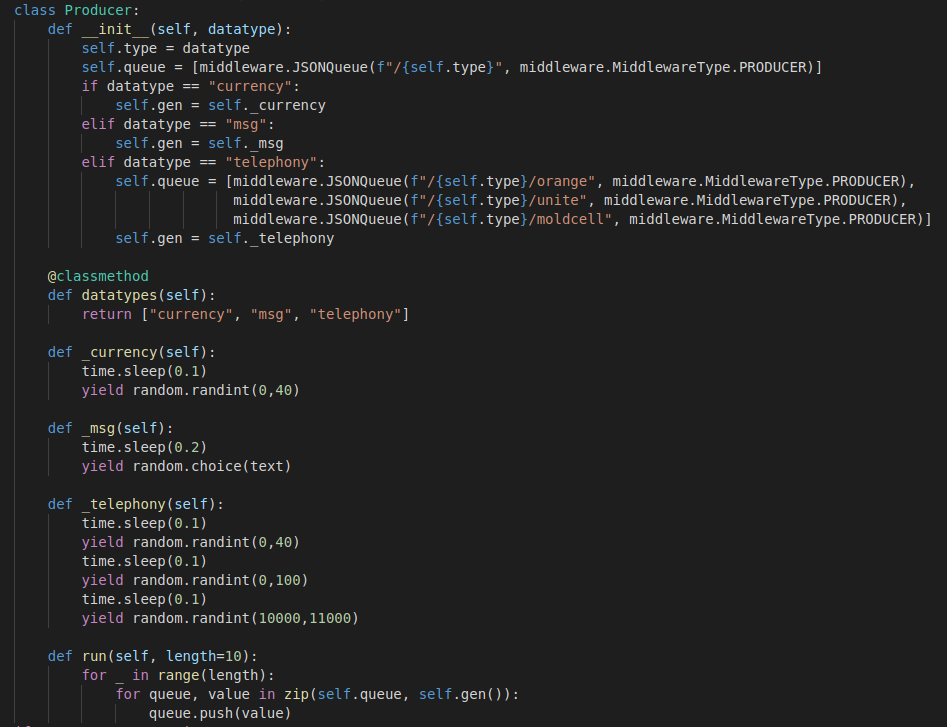
\includegraphics[scale=0.3]{producer}
	\caption{producer.py}\label{producer}
\end{figure}


\textbf{\\consumer.py}\\
\begin{figure}[!ht]
	\centering
	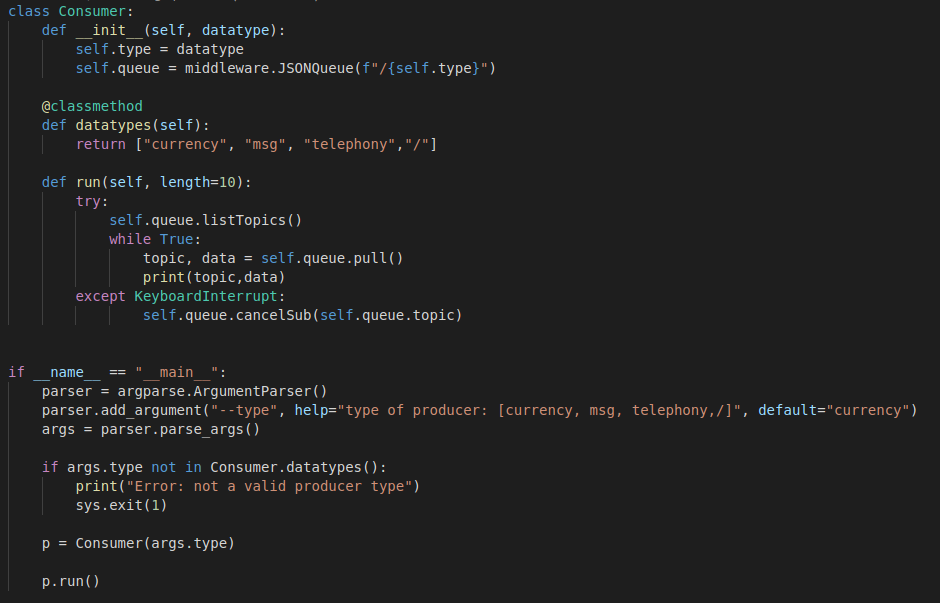
\includegraphics[scale=0.4]{consumer}
	\caption{consumer.py}\label{consumer}
\end{figure}

\clearpage